\chapterhead{6}{Finding What Went Missing}{Weighing after every step}\label{ch6}

A ledger at the end tells you \emph{that} something went missing. It cannot tell you \emph{where}. To find the step that lost something, weigh after \textbf{every} step and compare each result with what you expected.

\begin{center}
\sffamily\small\renewcommand{\arraystretch}{1.5}
\begin{tabular}{@{}p{3.4cm}p{3.7cm}p{3.7cm}@{}}
\toprule
\textbf{Model} & \textbf{What it keeps} & \textbf{What it drops}\\
\midrule
A mixture as parts & the weight of each part & how it looked\\
A sieve or magnet & the split by size or by steel & bits that get stuck\\
A solution & the total weight & where the salt sits\\
A filter & what is too big to pass & anything dissolved\\
A step ledger & where the loss happened & the cause of the loss\\
\bottomrule
\end{tabular}
\end{center}

\begin{tryit}{A step ledger}
Make a mixture of 12~g clips, 30~g pebbles and 58~g sand (100~g in all). Separate it in two steps: magnet, then sieve. Weigh the mixture and every product after each step. Fill in what you expected and what you found.\par\medskip
\renewcommand{\arraystretch}{1.6}
\begin{tabular}{|l|c|c|c|}
\hline
\textbf{After} & \textbf{Expected (g)} & \textbf{Weighed (g)} & \textbf{Gap (g)}\\ \hline
Start & 100 & & \\ \hline
Magnet: clips out, rest left & & & \\ \hline
Sieve: pebbles on it, sand through & & & \\ \hline
\end{tabular}
\end{tryit}

\begin{worked}{Practice numbers, not from a real test}
Start: 100~g. After the magnet: clips 12~g and rest 88~g. Expected 88, weighed 88. No gap.\\
After the sieve: pebbles 30~g on the sieve, sand through into the bowl 53~g. Expected $58$, weighed 53. The gap is 5~g.\\
The gap appeared at the \emph{sieve step}. A little pile of sand was on the table beside the bowl.
\end{worked}

\begin{center}
\sffamily\small\renewcommand{\arraystretch}{1.5}
\begin{tabular}{@{}lrrr@{}}
\toprule
\textbf{After} & \textbf{Expected} & \textbf{Weighed} & \textbf{Gap}\\
\midrule
Start & 100 & 100 & 0\\
Magnet & 88 & 88 & 0\\
Sieve (sand through) & 58 & 53 & \textbf{5}\\
\bottomrule
\end{tabular}
\end{center}

\begin{multix}[hmm]\multixbot[hmm]\tcblower
The total was 5 grams short at the end, so 5 grams of sand turned to dust and vanished. A loud thought, but a good one. Is it?
\end{multix}

\trust{We weighed after every step, so each step could be checked against what it should have produced.}
{Only the sieve step showed a gap, and the pile of sand on the table matched its size.}
{That every small gap has such a visible cause. Gaps of 1~g or less are within the scale's error and cannot be traced.}

\begin{keepbox}
We turned a separation into a table of weights. \textbf{We kept} \wline[3.4cm] \textbf{and we set aside} \wline[3.4cm].
\end{keepbox}

\clearpage

\begin{puzzle}{Find the step}
Start 80~g. After step 1 expected 70, weighed 70. After step 2 expected 49, weighed 44. At which step did the gap appear? \wline[2cm] How big? \wline[1.6cm]~g
\end{puzzle}

\begin{puzzle}{Fill the table}
Start 90~g. The magnet takes out 15~g. What do you expect to be left? \wline[1.6cm]~g
\end{puzzle}

\begin{puzzle}{Within error?}
A gap of 1~g appeared at a step weighed on a scale with 1~g error. Can you tell where it went? \wline[2cm] Why or why not? \wline[4cm]
\end{puzzle}

\begin{puzzle}{Check one step}
Why is weighing after every step better than weighing only at the end? \wline[6cm]
\end{puzzle}

\begin{puzzle}{Clue}
A 5~g gap appeared at the sieve. Name two clues you would look for. \wline[6cm]
\end{puzzle}

\clearpage

\begin{puzzle}{Add the table}
A table shows gaps of 0, 2 and 1~g after three steps. Total gap? \wline[1.6cm]~g
\end{puzzle}

\begin{puzzle}{Model or real?}
Write M for model and R for real thing.\\
(a) the table of weights \wline[1cm] \quad (b) the pile of sand on the table \wline[1cm] \quad (c) a circle with 88 in it \wline[1cm]
\end{puzzle}

\begin{puzzle}{Which question?}
The ledger can answer ``where did the weight go?'' Can it answer ``why did the sand spill?'' \wline[2cm] What else would you need? \wline[4cm]
\end{puzzle}

\begin{puzzle}{Unfair ledger}
Ben weighed after the magnet on one scale and after the sieve on another. Why can that mislead? \wline[6cm]
\end{puzzle}

\clearpage

\begin{puzzle}{Recount}
Clips 12~g, pebbles 30~g and sand 53~g. Total \wline[1.6cm]~g
\end{puzzle}

\begin{puzzle}{Wrap}
The student wrote ``5 g of sand vanished''. Wrap it with a better claim. \wline[6cm]
\end{puzzle}

\begin{puzzle}{A good habit}
Write one habit from this book that makes a mixture test more trustworthy. \wline[6cm]
\end{puzzle}

\begin{puzzle}{Missing step}
A student weighed the whole, then the clips, then the sand, and then said the salt was ``what is left''. What could go wrong? \wline[6cm]
\end{puzzle}

\clearpage

\begin{puzzle}{Draw the step circles}
Draw the magnet step as circles: a whole of 90~g, clips of 15~g, and the rest.
\begin{center}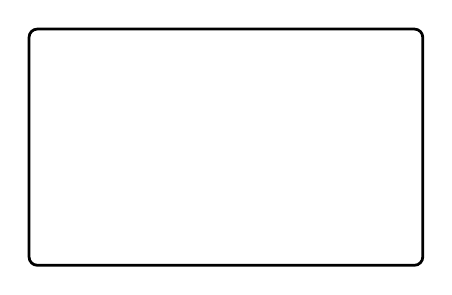
\begin{tikzpicture}\draw[line width=1pt,rounded corners=3pt] (0,0) rectangle (5,3); \end{tikzpicture}\end{center}
\end{puzzle}

\begin{puzzle}{Draw the gap}
Draw the sieve step with a 5~g gap as its own circle.
\begin{center}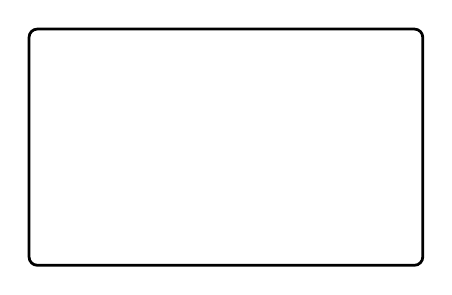
\begin{tikzpicture}\draw[line width=1pt,rounded corners=3pt] (0,0) rectangle (5,3); \end{tikzpicture}\end{center}
\end{puzzle}

\begin{puzzle}{Draw the wrap}
Draw a circle around ``5~g vanished'' and write the corrected claim outside it.
\begin{center}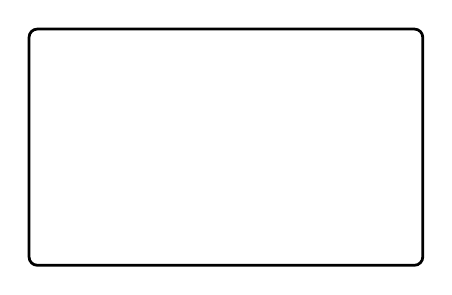
\begin{tikzpicture}\draw[line width=1pt,rounded corners=3pt] (0,0) rectangle (5,3); \end{tikzpicture}\end{center}
\end{puzzle}

\clearpage
\thispagestyle{fancy}\label{slop}
\subhead{Slop check}
Slop is hasty, gaudy work that forgot to take care. It can be made by a person or a machine, quickly or slowly. What matters is whether the work shows care for three things:
\begin{itemize}[leftmargin=1.6em]
\item \textbf{Salient:} Is the main point easy to see?
\item \textbf{Simple:} Is there anything that does nothing but get in the way?
\item \textbf{Relevant:} Does everything on the page help answer the question?
\end{itemize}

Here is a hasty poster about a separation. Study it, then decide what is wrong.

\begin{center}
\begin{tikzpicture}[scale=0.97]
  \fill[yellow!40,draw=purple!80!black,line width=3pt] (0,0) rectangle (11.4,7.6);
  \node[star,star points=12,fill=red!60,draw=blue,line width=2pt,minimum size=2.2cm,font=\bfseries\scriptsize,rotate=10,text=yellow] at (1.4,6.2) {WOW!!!};
  \node[font=\itshape\bfseries\Large,text=teal,rotate=-4] at (6.4,6.8) {MiXiNg Is MaGiC};
  \node[font=\ttfamily\tiny,text=orange] at (6.4,6.15) {(stuff maybe? who knows)};
  \foreach \x/\h/\c in {3/1.2/red,5.3/3.2/blue,7.6/5.0/green}{
    \fill[\c,draw=black] (\x,0.9) rectangle (\x+1.3,0.9+\h);
  }
  \node[font=\tiny,text=black,rotate=60] at (9.8,3) {number number number};
  \foreach \x/\y in {1.2/1.5,1.6/4.2,10.2/5.6,0.8/3}{\node[star,star points=5,fill=yellow,draw=red,minimum size=0.6cm] at (\x,\y) {};}
  \node[font=\tiny,text=lime!50!black] at (5.4,0.45) {sort it!!!  best sorting ever!!!  wow  wow};
\end{tikzpicture}
\end{center}

\begin{slopbox}
\textbf{(a)} What is the poster's main point? Can you tell?\\[3pt]\rule{\linewidth}{0.5pt}\\[6pt]
\textbf{(b)} Name two things that are not simple, because they only distract.\\[3pt]\rule{\linewidth}{0.5pt}\\[6pt]
\textbf{(c)} Name two things that are missing, so the bars cannot be read.\\[3pt]\rule{\linewidth}{0.5pt}\\[6pt]
\textbf{(d)} Which part is not relevant to mixtures at all?\\[3pt]\rule{\linewidth}{0.5pt}
\end{slopbox}

\clearpage
\thispagestyle{fancy}
\subhead{Now you try}
On a separate sheet, redraw a clear bar chart of the three parts of the mixture: clips 10~g, sand 49~g and salt 19~g. Give it a title, label the axes with units, use one or two calm colours, and delete everything that does not help. Check it against the three words: salient, simple, relevant.

\begin{center}
\begin{tikzpicture}
  \draw[ink!70,line width=1pt,rounded corners=3pt] (0,0) rectangle (11.4,1.0);
  \node[font=\sffamily\small,anchor=west] at (0.2,0.5) {Title:};
  \draw[line width=1.3pt] (1,1.6) -- (1,9.6);\draw[line width=1.3pt] (1,1.6) -- (11,1.6);
  \foreach \y in {2.6,3.6,...,8.6}{\draw[gray!40] (1,\y) -- (11,\y);}
  \node[font=\sffamily\scriptsize,rotate=90] at (0.3,5.6) {label and unit here};
  \node[font=\sffamily\scriptsize] at (6,1.3) {label what the axis stands for};
\end{tikzpicture}
\end{center}

\clearpage
\thispagestyle{fancy}
\subhead{What did we keep, across the whole book?}
For each chapter, say one thing that was simplified, what was kept, and what was set aside. A sample is done for you.

\renewcommand{\arraystretch}{2.3}
\begin{center}\sffamily\scriptsize
\begin{tabularx}{\textwidth}{|>{\bfseries}p{2.1cm}|X|X|X|}
\hline
\textbf{Chapter} & \textbf{What we simplified} & \textbf{What we kept} & \textbf{What we set aside} \\ \hline
1 What a mixture is & a bowl of things as weights & the weight of each part & how it looked \\ \hline
2 Sieves and magnets & a tool as one difference & the split by size or steel & bits that got stuck \\ \hline
3 Salt that disappears & dissolved salt as a weight & the total weight & where the salt sits \\ \hline
4 Muddy water & a filter as a catcher & the mud's weight & dissolved things \\ \hline
5 Separating everything & a plan as ordered steps & the order and the total & small losses \\ \hline
6 Missing weight & & & \\ \hline
\end{tabularx}
\end{center}

\begin{multix}[wow]\multixbot[wow]\tcblower
Everything you weighed in this book was a simplification of something. A model is allowed to drop things, as long as you say which. Next time something seems to vanish, you will know to weigh again.
\end{multix}

\clearpage
\thispagestyle{fancy}
\subhead{Write a separation report}
\begin{tcolorbox}[enhanced,colback=white,colframe=ink!60,boxrule=1pt,arc=2mm,left=8pt,right=8pt,top=5pt,bottom=5pt]
\sffamily\small
\begin{enumerate}[leftmargin=1.6em,itemsep=0.2em]
\item \textbf{What I looked at.}
\item \textbf{What I changed, measured and kept the same.}
\item \textbf{My readings.} All of them.
\item \textbf{My answer.} With the gap named.
\item \textbf{What I kept and what it hides.}
\end{enumerate}
\end{tcolorbox}
\vspace{4pt}
Pick one separation from this book and write a report on it. Use the lines below.\par\medskip
\foreach \i in {1,...,12}{\rule{\linewidth}{0.4pt}\\[18pt]}
\clearpage

\thispagestyle{fancy}
\subhead{Tests to try}
Pick one and design it with the habits from this book: change one thing, keep the rest the same, repeat, and weigh every step.
\begin{enumerate}[leftmargin=1.6em,itemsep=0.5em]
\item Does warm water dissolve more salt than cold water?
\item Does stirring change how fast sugar dissolves?
\item Which paper filters muddy water clearest: coffee filter, paper towel or cloth?
\item Can you separate rice, lentils and sand with a sieve alone?
\item How much of a salt crust can you get back from 100~g of salt water?
\item Which kitchen mixture is easiest to take apart, and which is hardest?
\end{enumerate}
\medskip
Write the test you pick:\par\medskip
\foreach \i in {1,...,6}{\rule{\linewidth}{0.4pt}\\[16pt]}
Change: \wline[3cm] Measure: \wline[3cm] Keep the same: \wline[3cm]
\clearpage

\thispagestyle{fancy}
\subhead{A week of mixtures}
Each day, notice one mixture and say how you could take it apart.\par\medskip
\renewcommand{\arraystretch}{3.2}
\begin{tabularx}{\linewidth}{|>{\sffamily\small\bfseries}p{1.8cm}|X|X|}
\hline
Day & The mixture & A tool I could use \\ \hline
Mon & & \\ \hline
Tue & & \\ \hline
Wed & & \\ \hline
Thu & & \\ \hline
Fri & & \\ \hline
Sat & & \\ \hline
Sun & & \\ \hline
\end{tabularx}
\clearpage

\thispagestyle{fancy}
\subhead{Questions I still have}
Write what you still wonder about mixtures. Then pick one and think how to test it.\par\medskip
\foreach \i in {1,...,16}{\rule{\linewidth}{0.4pt}\\[16pt]}
\clearpage
